We measure lithium 6707.79 \r{A} equivalent widths from ARCES spectra so that we can use them and the python package \texttt{BAFFLES} \citep{2020ApJ...898...27S} to derive age posteriors. \rev{First, we bring the spectrum to the approximate rest frame using the \textit{Gaia} DR3 radial velocity measurement \citep{2023A&A...674A...1G} for the star and correct for the Earth's motion by applying a barycentric correction.} To find the lithium 6707.79 \r{A} feature and measure its equivalent width, we fit a double Gaussian with a slope to the spectrum with the functional form
\begin{equation}
  \rev{f_{mod} = (m(\lambda-6707.0)+b)(C_{1}e^{-0.5(6707.79 -RV_{s}-\lambda)^{2}/\sigma^{2}}+C_{2}e^{-0.5(\lambda_{ref}-RV_{s}-\lambda)^{2}/\sigma^{2}})}
\end{equation}

\noindent where $\lambda$ is the wavelength array, $m$ and $b$ are the slope and intercept of the continuum; $\lambda_{ref}$ is the central wavelength of some reference feature; $C_{1}$ is the depth of the lithium feature; $C_{2}$ is the depth of the reference line; $\sigma$ represents the standard deviation of both Gaussians; $RV_{s}$ represents an additional radial velocity shift to the \textit{Gaia} DR 3 measurement. \rev{We include this additional RV offset term in our fit to account for potential orbiting companions or any radial velocity drift in ARCES.} For most stars, we adopt $\lambda_{ref} = 6705.1$  \r{A}, a prominent Fe line. For lower mass stars where the 6705.1 \r{A} Fe line is not present, we adopt $\lambda_{ref} =  6717.8$  \r{A}, a prominent Ca line. \rev{The reference line prevents the fit from selecting a value for the radial velocity, $RV_{s}$ that shifts another line (or noise trough) to the location of the lithium line. This also prevents the fit from adjusting the width of the lithium feature to match a noise trough.} This is especially useful in cases where the lithium line is weak or not detectable. When $\lambda_{ref} = 6705.1$ \r{A} we use the region of spectra from 6704 \r{A} to 6710  \r{A}. When $\lambda_{ref} = 6717.8$ \r{A} we use the region of the spectrum from 6706 \r{A} to 6720  \r{A}. Both of these regions fall on a single ARCES order.

Since the 6707.79 \r{A} feature is a blend of the $^6Li$ and $^7Li$ doublets, we find the effective center of the entire feature by fitting the double Gaussian to a narrow region of spectrum from 6704 \r{A} to 6710 \r{A} for several stars where $\lambda_{ref} = 6705.1$ \r{A} such that

\begin{equation}
 \rev{ f_{mod} = (m(\lambda-6707.0)+b)(C_{1}e^{-0.5(6707.79 + s-RV_{s}-\lambda)^{2}/\sigma^{2}}+C_{2}e^{-0.5(6705.105-RV_{s}-\lambda)^{2}/\sigma^{2}})}
\end{equation}
 
\noindent Here, $s$ is the deviation of the center of the lithium feature from 6707.79 \r{A}.
 
 We use the python package \textit{emcee} \citep{2013PASP..125..306F} to run Markov Chain Monte Carlo (MCMC) fits on several spectra and found that $s$ for the best fit was consistently 0.0119 \r{A} regardless of spectral type, so we adopt 6707.819 \r{A} as the effective center of the lithium feature. %and change the functional form to
 
%\begin{equation}
 % f_{mod} = (m(\lambda-6707.0)+b)(C_{1}e^{((-0.5(6707.819 -RV_{s}-%\lambda)/\sigma)^{2}}+C_{2}e^{((-0.5(\lambda_{ref}-RV_{s}-\lambda)/\sigma))^{2}})
%\end{equation}\noindent for our double Gaussian model. 
With Equation 3 and \textit{emcee}, we run MCMC to find the best-fitting parameters and estimates of their uncertainties for each spectrum. The uncertainties in each pixel of the spectrum are assumed to follow a Poisson distribution and include estimates of the gain and read noise. 

\rev{First, we run a preliminary MCMC with 100 walkers and 10,000 steps to find good starting positions. Then, a second round of MCMC is run from these starting positions, with 100 walkers, for 50,000 steps with a 2,000 step burn-in, which was sufficient to achieve convergence for most stars. 16 stars with non-detections required 100,000 steps with a 10,000 step burn-in, and 2 additional stars required 400,000 steps with a 200,000 step burn-in. We assessed convergence both by visual inspection and by comparing the posteriors at the start and end of each chain. We also compute the integrated autocorrelation time (IAT) of our chains, which has a maximum value of 1.2; we therefore estimate that there are at least 35,000 independent samples of the posterior, consistent with the start and end of each chain being independent. Comparing the median of each parameter at the first 10\% of each chain to the final 10\% we find the largest fractional difference to be 9\%. A similar test comparing the standard deviation from the first and last 10\% yields a maximum fractional difference of 6\%. These results are consistent with convergence.} To calculate the lithium equivalent width, we integrate a Gaussian with parameters from the MCMC chains 
 %
\begin{equation}
 \Sigma_{Li} = \sqrt{2\pi}C_{1}\sigma
\end{equation} which we converted to an equivalent width by scaling the area by the height of the nearby continuum, $H$
\begin{equation}
 EW_{Li} = \frac{\sqrt{2\pi}C_{1}\sigma}{H}
\end{equation}

To find the height of the nearby continuum, we evaluate a line defined by the slope ($m$) and intercept ($b$) of the fit at 6707.819 \r{A} (the center of the lithium feature). We use our chains to compute the posterior on equivalent width and report the median. We take the standard deviation of the equivalent width posterior from the converged chain as our uncertainty.


For stars that do not have a clear lithium feature, we use the same MCMC fitting method to calculate upper limits on the lithium equivalent width. For upper limits, $C_{1}$ in Equation 3 approaches zero, and $\sigma$ and $RV_{s}$ are set almost entirely by the reference line. We identify upper limits by measuring the skew of the equivalent widths' distribution. If the skew exceeds 0.225 or the mean of the distribution is below 5 m\r{A}, we flag the spectrum as a candidate upper limit. We confirm our upper limit selection by visually inspecting the spectrum. We calculate the 1, 2, and 3$\sigma$ upper limits by calculating the 68th, 95th, and 99.7th percentiles of the cumulative distribution function. We over-plot Gaussians with $\sigma$ determined by the reference line and depths set by the 1, 2, and 3$\sigma$ upper limits to visually assess the corresponding upper limit on the equivalent width. We report the $2\sigma$ upper limits.

We calculate the equivalent width for each star using both spectral orders that include the lithium 6707.8 \r{A} feature. \rev{We adopt the equivalent width measurement or upper limit from the order/observation combination that yields the best fit to the data. This is generally the segment with the highest signal-to-noise ratio and no cosmic rays. We confirm our selection by visually assessing the fits. Each fit typically returns similar measurements of the lithium equivalent width, with error bars scaling with SNR as we would expect.} Figure \ref{li_spec_examples} shows examples of a lithium detection and a lithium upper limit determined from this process.



\begin{figure*}[ht !]
\centering
 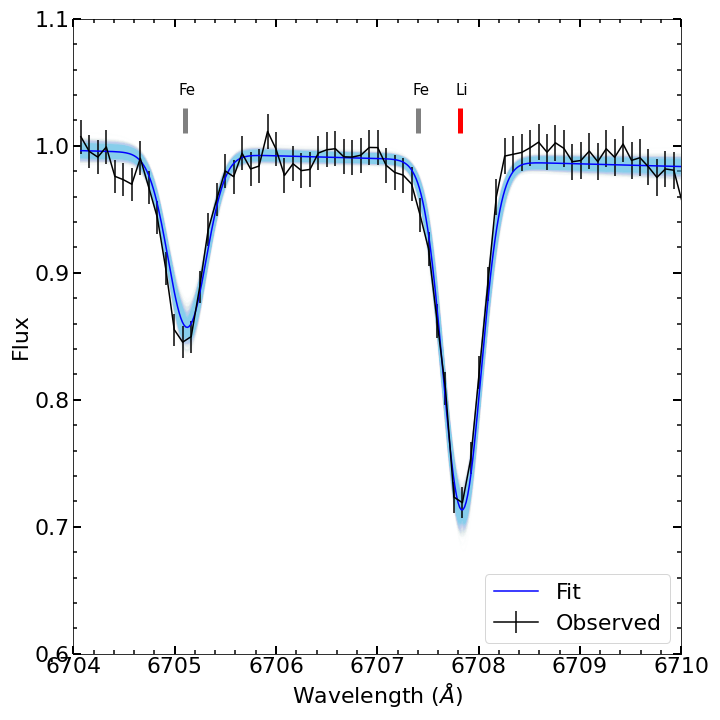
\includegraphics[scale = 0.3]{Li_fit_example.png}
 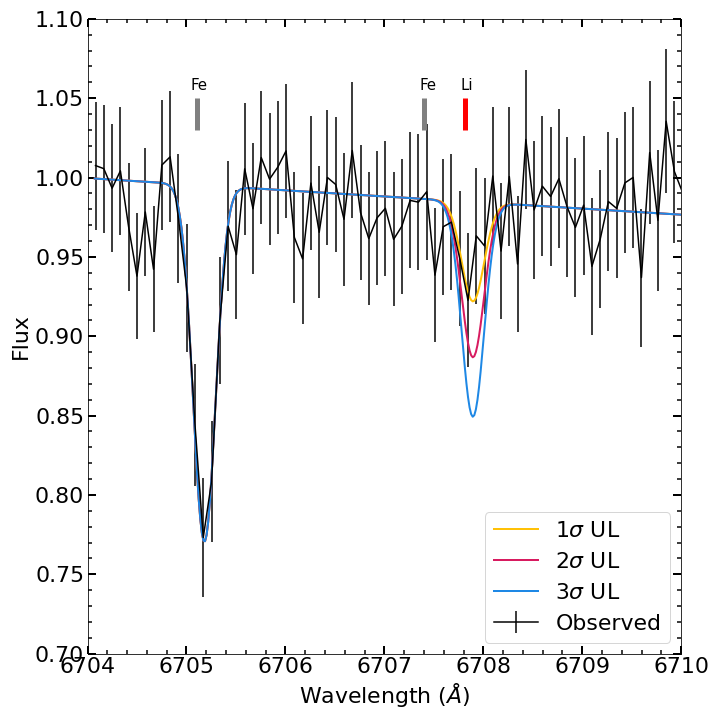
\includegraphics[scale = 0.3]{Li_UL_example.png}
 \caption{Our double Gaussian fitting technique allows us to robustly measure lithium equivalent widths and, in cases where lithium is not detected, place upper limits on the lithium equivalent widths. {\bf Left:} A spectrum of HIP 41277 ($SNR\sim75$) covers both the Fe 6705.1 \r{A} line (used as a reference line) and the Li 6707.79 \r{A} feature. Black points with error bars are the APO/ARCES data, the dark blue line represents the highest likelihood fit from the MCMC, and the light blue lines are random draws from the posterior. We find a lithium equivalent width for HIP 41277 of $125\pm{5}$ m\r{A}. {\bf Right:} An example spectrum ($SNR\sim30$) of an upper limit for lithium, from HIP 110663. Data are again black points with error bars, while yellow, red, and blue represent 1, 2, and 3$\sigma$ upper limits. We find a 2$\sigma$ upper limit of $30$ m\r{A} for HIP 110663, which we use to set a lower limit on the age of the star.}
 \label{li_spec_examples}
 
\end{figure*}

\begin{figure*}[ht!]
\centering
 
 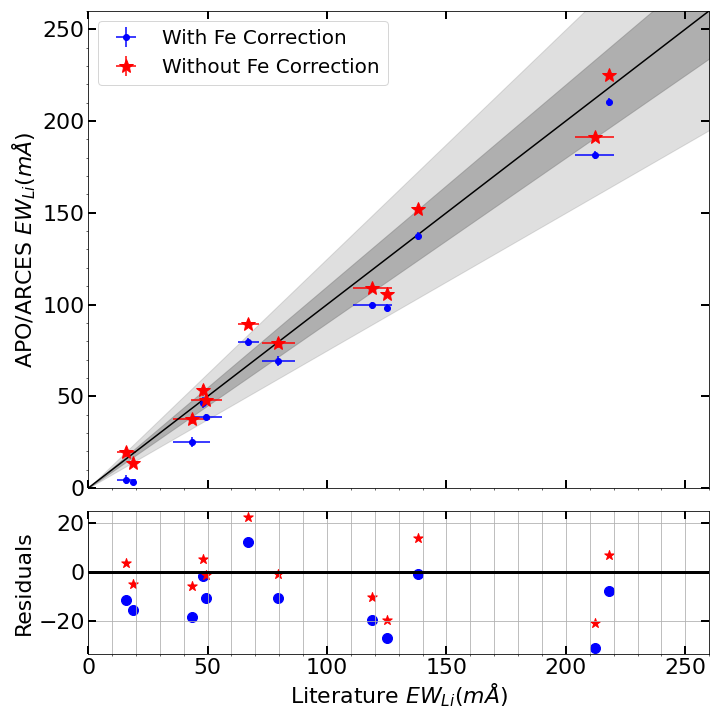
\includegraphics[scale = 0.375]{Lithium_check.png}
 \caption{Comparing our lithium equivalent width measurements to results from the literature for 12 stars (red stars) shows good agreement. The black line shows the 1-to-1 relation, with $\pm10\%$ in dark gray and $\pm25\%$ in light gray. We find that applying a correction for the 6707.4 \r{A} iron line \citep{1993AJ....105.2299S} results in a systematic underestimate of the literature abundances (blue points). We conclude that our Gaussian fitting technique is robust to contamination from the 6707.4 \r{A} iron line, so we do not include an additional correction to our reported equivalent width values. We take literature lithium equivalent widths for HIP 104075, HIP 105232, HIP 113905, HIP 35628, HIP 97779 from \cite{2009A&A...504..829G}, HIP 115147, HIP 43410, HIP 52462, HIP 71631 from \cite{2003A&A...399..983W}, HIP 42438 from \cite{2007AJ....133.2524W}, and HIP 43726 from \cite{2005PASJ...57...45T}.}
 \label{li_check}
 
\end{figure*}
For stars with large amounts of lithium or high rotational velocities, the lithium 6707.8 \r{A} feature can be blended with the 6707.4 \r{A} Fe line. Past work has introduced a correction factor to equivalent widths to subtract the contribution of the iron line from the blended equivalent width. For example \cite{1993AJ....105.2299S} calculate iron 6707.4 \r{A} equivalent widths as a function of $B-V$, and subtract this from their blended equivalent widths. Similar methods are used by \cite{1993ASSL..183..303F, 2003A&A...399..983W, 2005PASJ...57...45T, 2007AJ....133.2524W, 2009A&A...504..829G}. To assess the degree to which including an iron blend correction improves our lithium equivalent width measurements, we compiled literature values where available for our target stars and S-value calibration targets (discussed below) from \cite{2013A&A...551L...8P}. In  Figure \ref{li_check}, we compare our measured lithium equivalent widths with and without the \cite{1993AJ....105.2299S} correction to these literature values for 12 stars. We find that our method with no correction applied yields more consistent equivalent widths compared to these literature values. Applying the \cite{1993AJ....105.2299S} correction systematically under-predicts the literature values. We attribute this to our method of fitting a Gaussian to the full absorption profile and taking the integral of the Gaussian, rather than summing \rev{fluxes in a specific wavelength range} directly from the spectrum. As a result, since the asymmetric wing from the iron line introduces a negligible effect on the final equivalent width, we do not apply a correction to our measured equivalent widths. 

\rev{To ensure there are no systematic offsets in our lithium fitting technique, we inject a Gaussian of a given equivalent width into an ARCES spectrum with no detectable lithium. Then we feed the injected spectrum through our fitting routine and recover the equivalent width. We conduct this test on five spectra with moderate to high signal-to-noise corresponding to stars at a range of spectral types. For each star, we repeat the injection/recovery test for 13 different values of injected lithium equivalent widths from 5-100 m\r{A}. Figure \ref{recovery} compares the recovered equivalent widths to the injected lines, which agree to $\lesssim$1 m\r{A}, well within the reported error bars for each measurement. The main source of this disagreement is noise in each spectrum with the noise being on average slightly above or slightly below the continuum at the location of the lithium line, resulting in a slight underestimate or overestimate of the equivalent width, respectively.}

\begin{figure*}[ht!]
\centering
 
 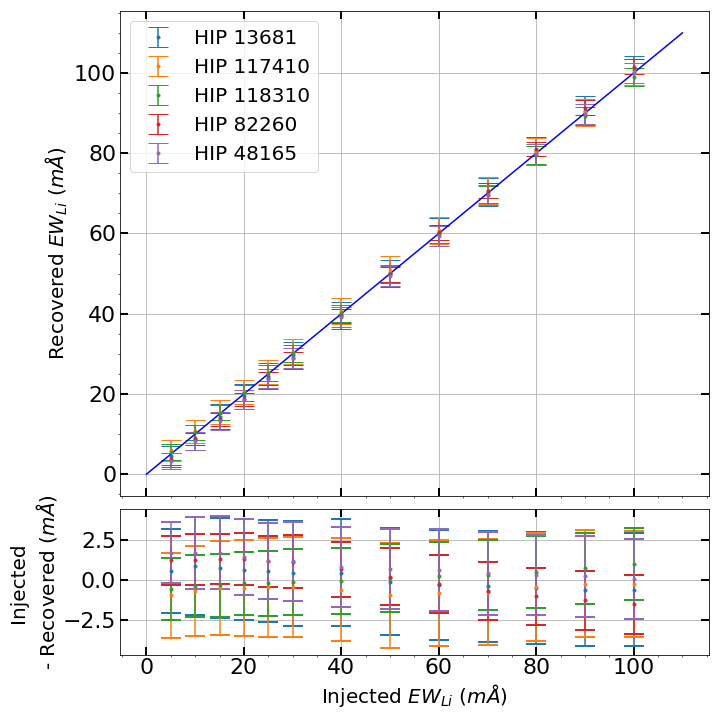
\includegraphics[scale = 0.375]{injection_recovery.png}
 \caption{\rev{We confirm that our lithium fitting routine reliably recovers accurate equivalent widths with injection/recovery tests on 5 stars. We chose these stars since they had no detectable lithium, and because they cover a range of SNR and spectral types. The recovered equivalent widths are all within $\lesssim$1 m\r{A} of the injected value, and consistent with reported error bars.}}
 \label{recovery}
 
\end{figure*}
\rev{We calculate age posteriors from lithium equivalent widths and uncertainties for our target stars using Bayesian Ages For Field LowEr-mass Stars (\texttt{BAFFLES}) \citep{2020ApJ...898...27S}. \texttt{BAFFLES} utilizes a Bayesian framework that is calibrated on stars in clusters and associations of known ages. Functional forms were fit both to lithium equivalent width as a function of $B-V$ for each calibration cluster, and the intrinsic scatter in equivalent width. Final age posteriors represent a combination of the astrophysical scatter in the age/equivalent width relation and the measurement error \citep{2020ApJ...898...27S}. \texttt{BAFFLES} uses a uniform star formation history as the age prior. The uncertainty on age is largely driven by the observed astrophysical scatter in lithium equivalent width at a constant age, with a much smaller contribution from the measurement uncertainty for a single star.} \texttt{BAFFLES} is calibrated to calculate age posteriors from lithium for stars with $B-V$ between 0.35 and 1.9 from both measurements and upper limits. Figure \ref{li_post_example} shows an example \texttt{BAFFLES} posterior for HIP 41277, where an equivalent width of $125\pm{5}$ m\r{A} translates to an age posterior of $174^{+79}_{-77}$ Myr. We detect lithium in 26 stars, and determine upper limits for 140 stars; of the full sample, \rev{159} stars are in the \texttt{BAFFLES} $B-V$ range.  We report $B-V$, lithium equivalent width measurements (or upper limits), and \rev{median ages and confidence intervals} from \texttt{BAFFLES} (where applicable) for our sample in Table \ref{tab:lithium}.

\begin{figure*}[h!]
\centering
 
 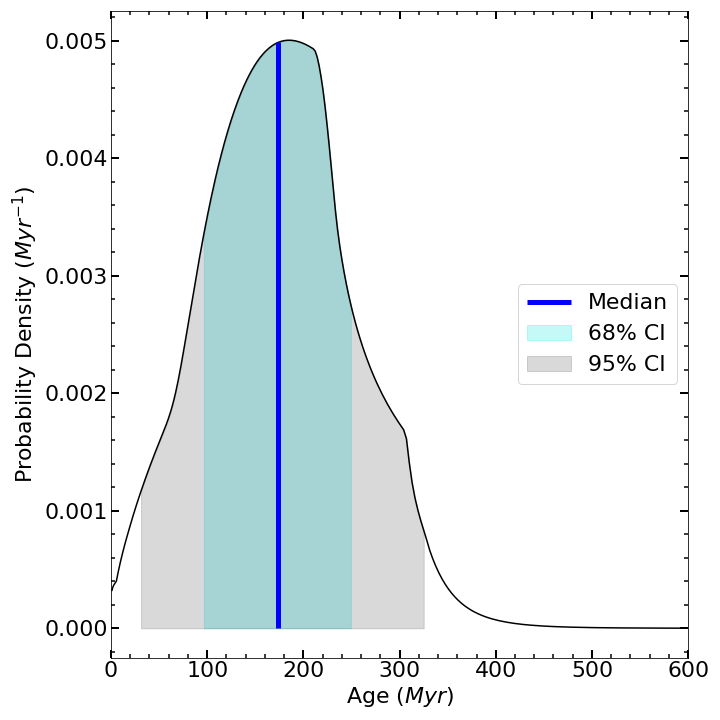
\includegraphics[scale = 0.375]{example_Li_post.png}
 \caption{An example of an age posterior for one star in our sample, HIP 41277, using \texttt{BAFFLES} \citep{2020ApJ...898...27S}. From an adopted B-V of $1.03\pm{0.015}$ and a lithium equivalent width of $125\pm{5}$ m\r{A}, we derive an age posterior with a median age of 174 Myr and $68\%$ confidence interval between 97 and 253 Myr. Lithium measurements \rev{and median ages, and $68\%$ and $95\%$ confidence intervals} for the full sample are reported in Table \ref{tab:lithium}.}
 \label{li_post_example}
 
\end{figure*}

\clearpage